\chapter{Control Design and Development}



\section{Controller}
The controller used to XXX is inspired in the paper \cite{QSC}. The objective of the controller is to determine the muscle excitation needed to stabilize the position of the wrist, see block diagram on Figure \ref{fig:BDC}

The desired arm configuration is the input of the controller. Using the Inverse of the Arm Statics model developed on section \ref{sec:spgp}, the desired torques needed to hold the arm in that static position are calculated. 

These torques are given to the inverse of the Muscle Torque Production model developed also on section \ref{sec:model}. The model outputs the corresponding muscle excitations for that static position. The muscle excitations are input to the Dynamic Arm Simulator that will calculate the dynamics of the arm following the Rosenbrock equation explained in section \ref{sec:dynamics}.

Finally the wrist position of the arm is calculated. The error between the desired and the current wrist position is given as input to a PID Controller. The PID controller calculate the corrective force needed to obtain the desired wrist position. The kinematic Jacobian (refer to section \ref{sec:torque}) is used to calculate the corresponding corrective torque. This torque is added to the desired torque output from the Inverse Arm Statics. The total torque is given as an input to the Inverse Muscle Torque model.

\begin{figure}[h!]
    \centering
    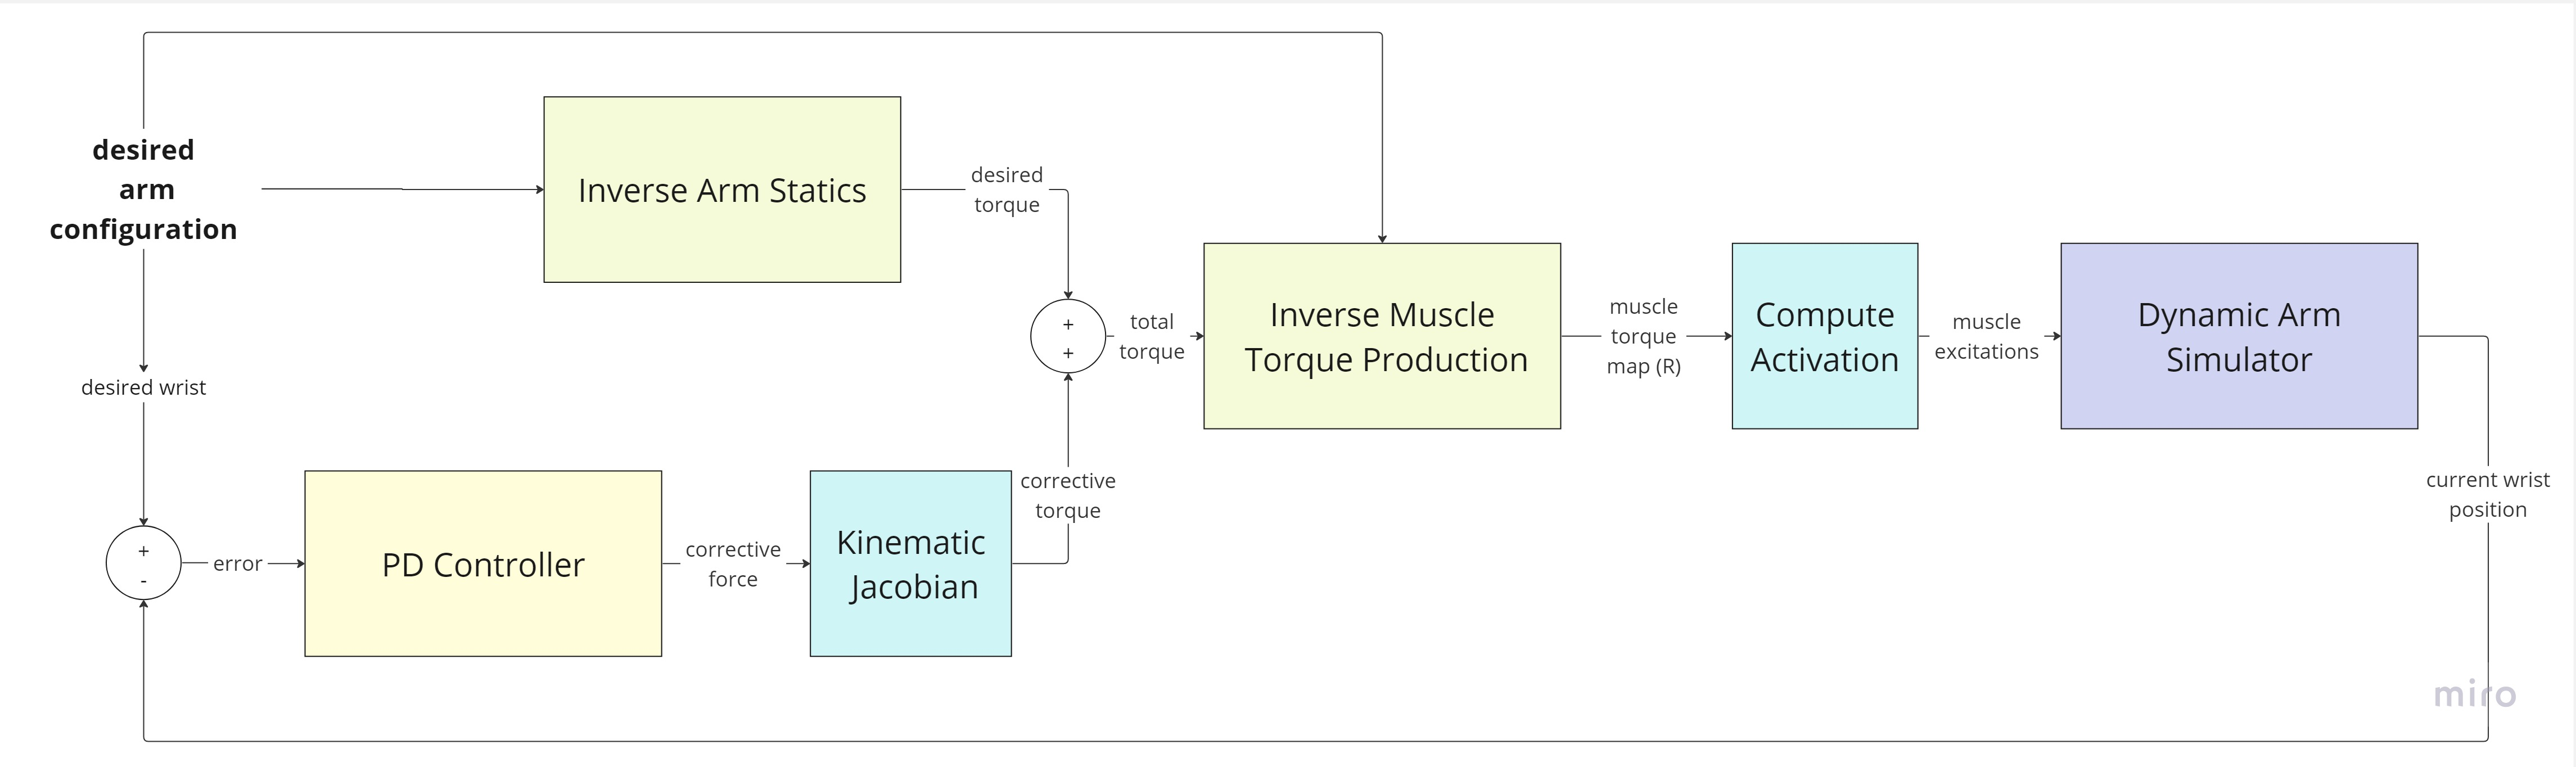
\includegraphics[width=0.9\textwidth]{Pictures/Controller/controller-diagram.jpg}
    \caption{Controller Block Diagram inspired in \cite{QSC}}
    \label{fig:BDC}
\end{figure}

% Explain Quasi-Static Controller and how you achieve this. 
% Diagram

\section{Path Following Quasi-Static Control Development }
\begin{figure}[h!]
    \centering
    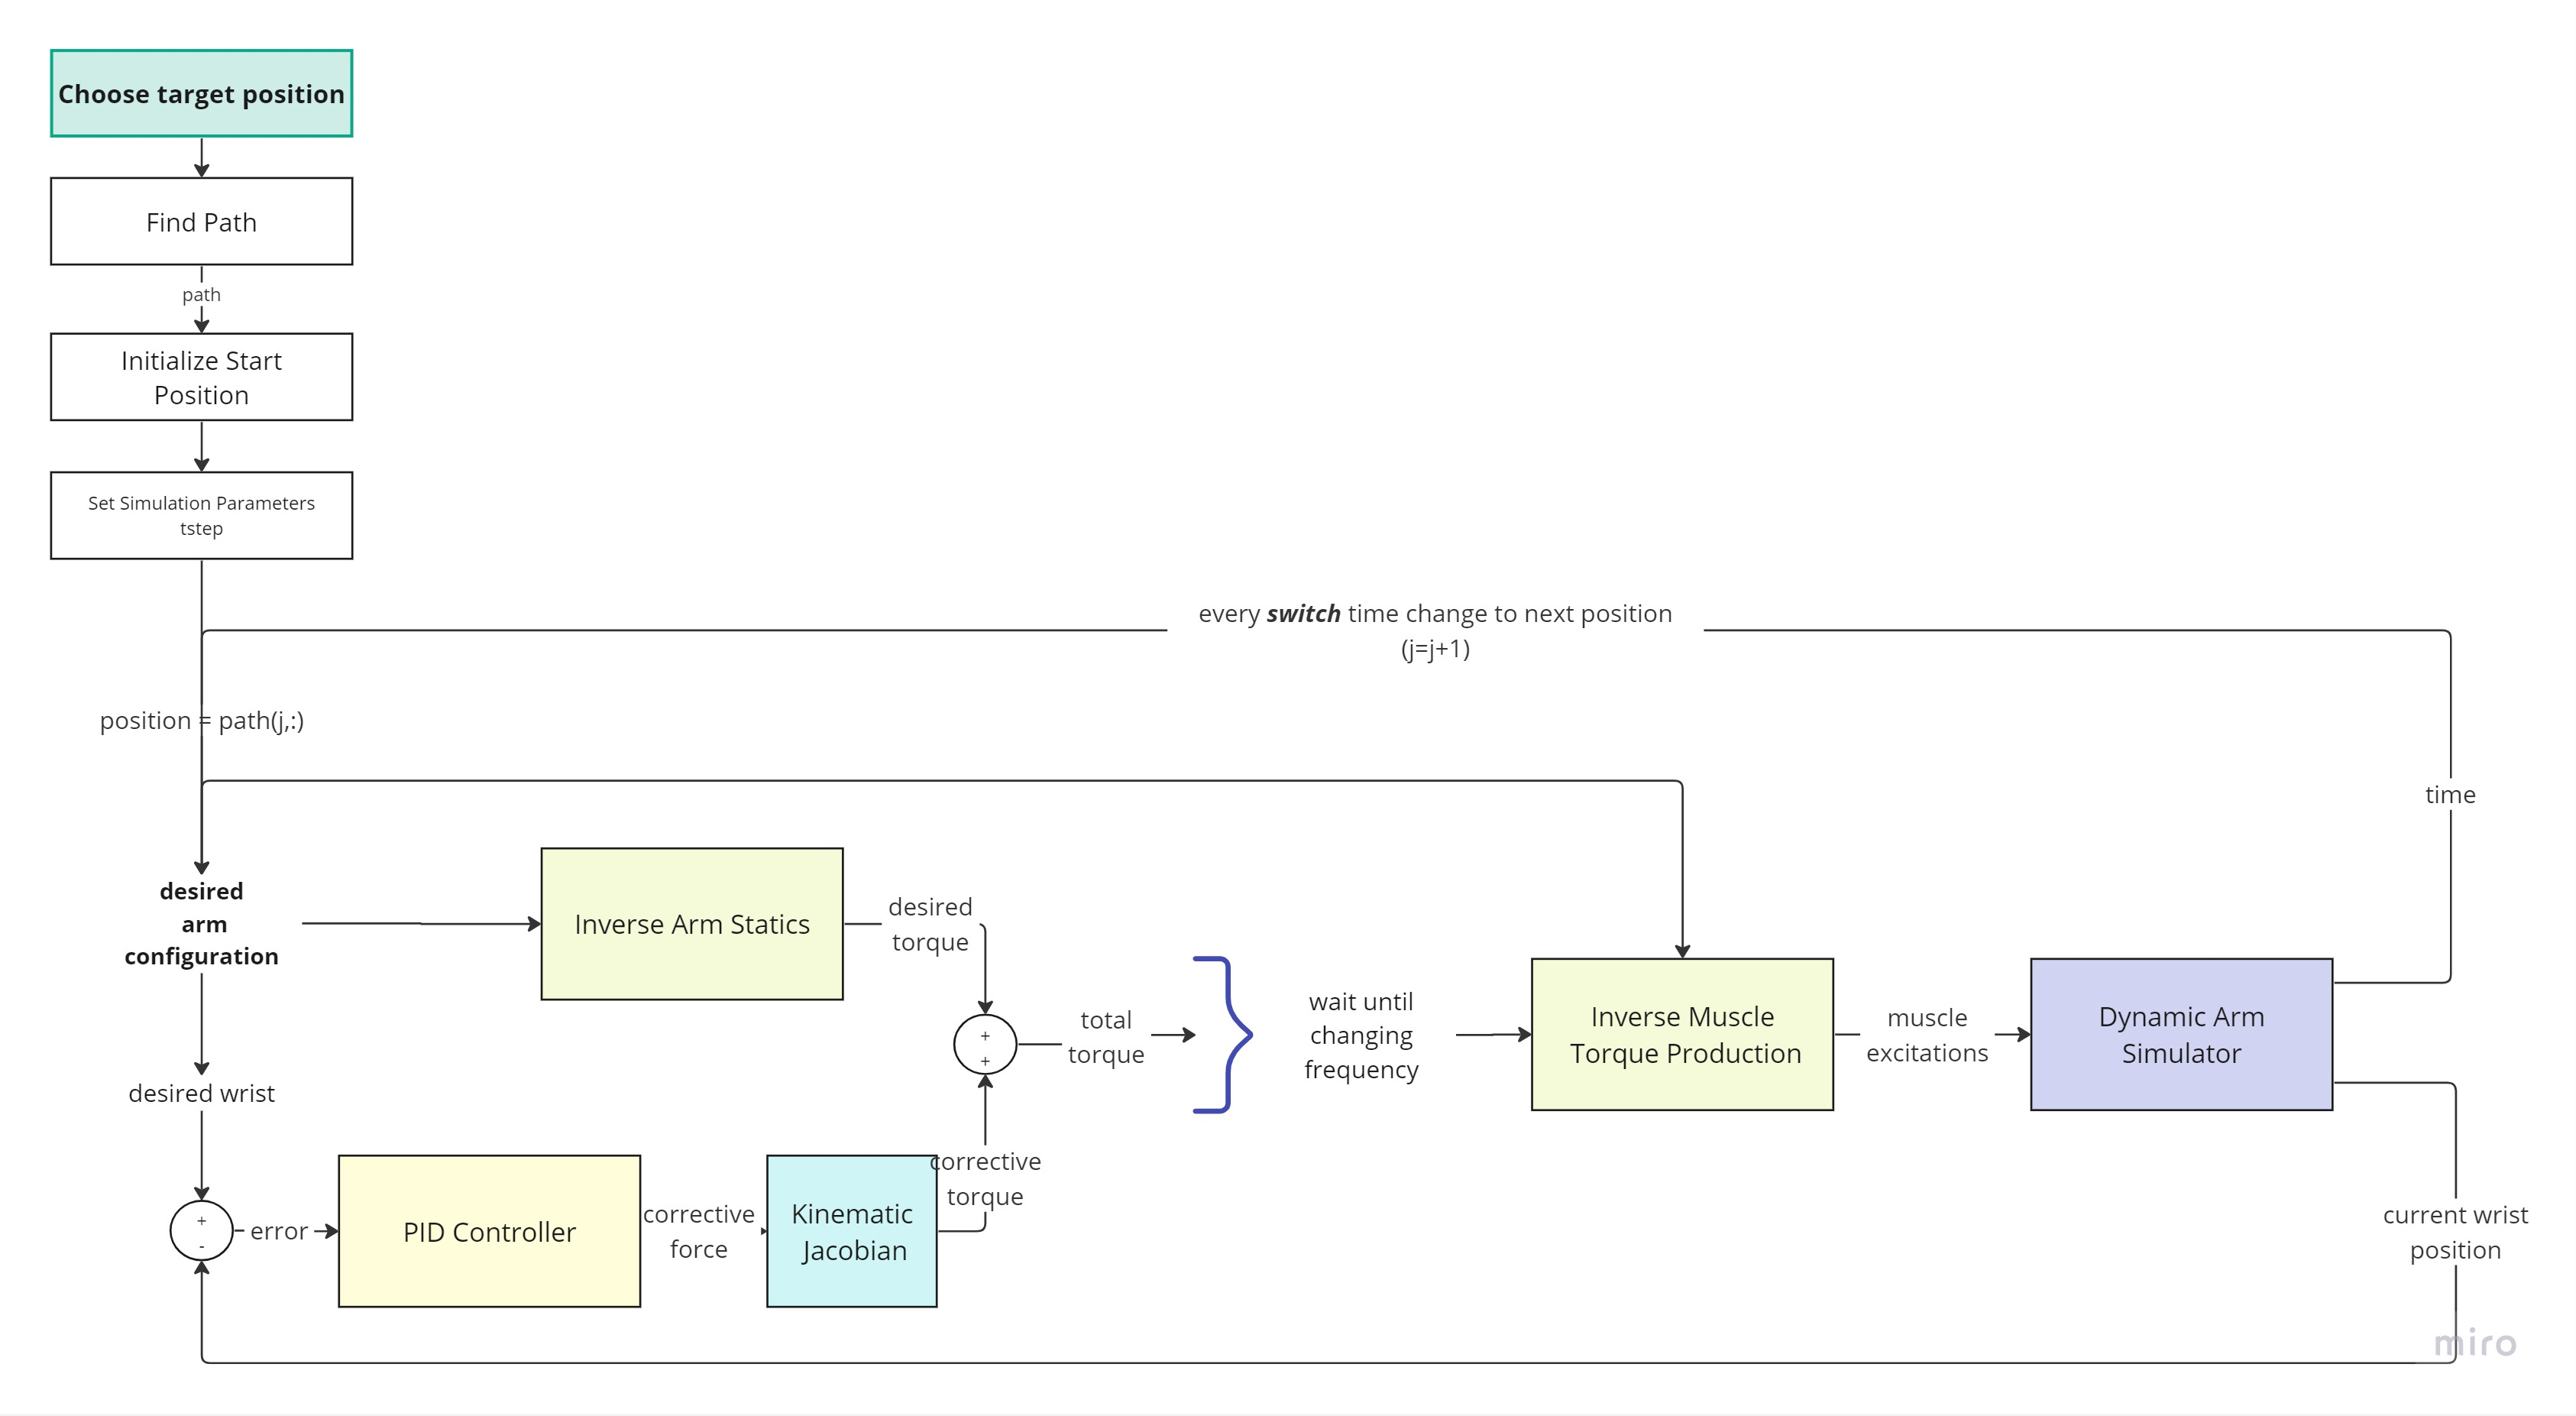
\includegraphics[width=0.9\textwidth]{Pictures/Controller/Quasi-Static Path Controller.jpg}
    \caption{Flow Diagram Quasi-Static Path Controller }
    \label{fig:PathController}
\end{figure}
% Describe the code
\section{EMG-Influenced Control Development}

\newpage
\begin{landscape} % Start landscape page
  \begin{figure}[h!]
    \centering
    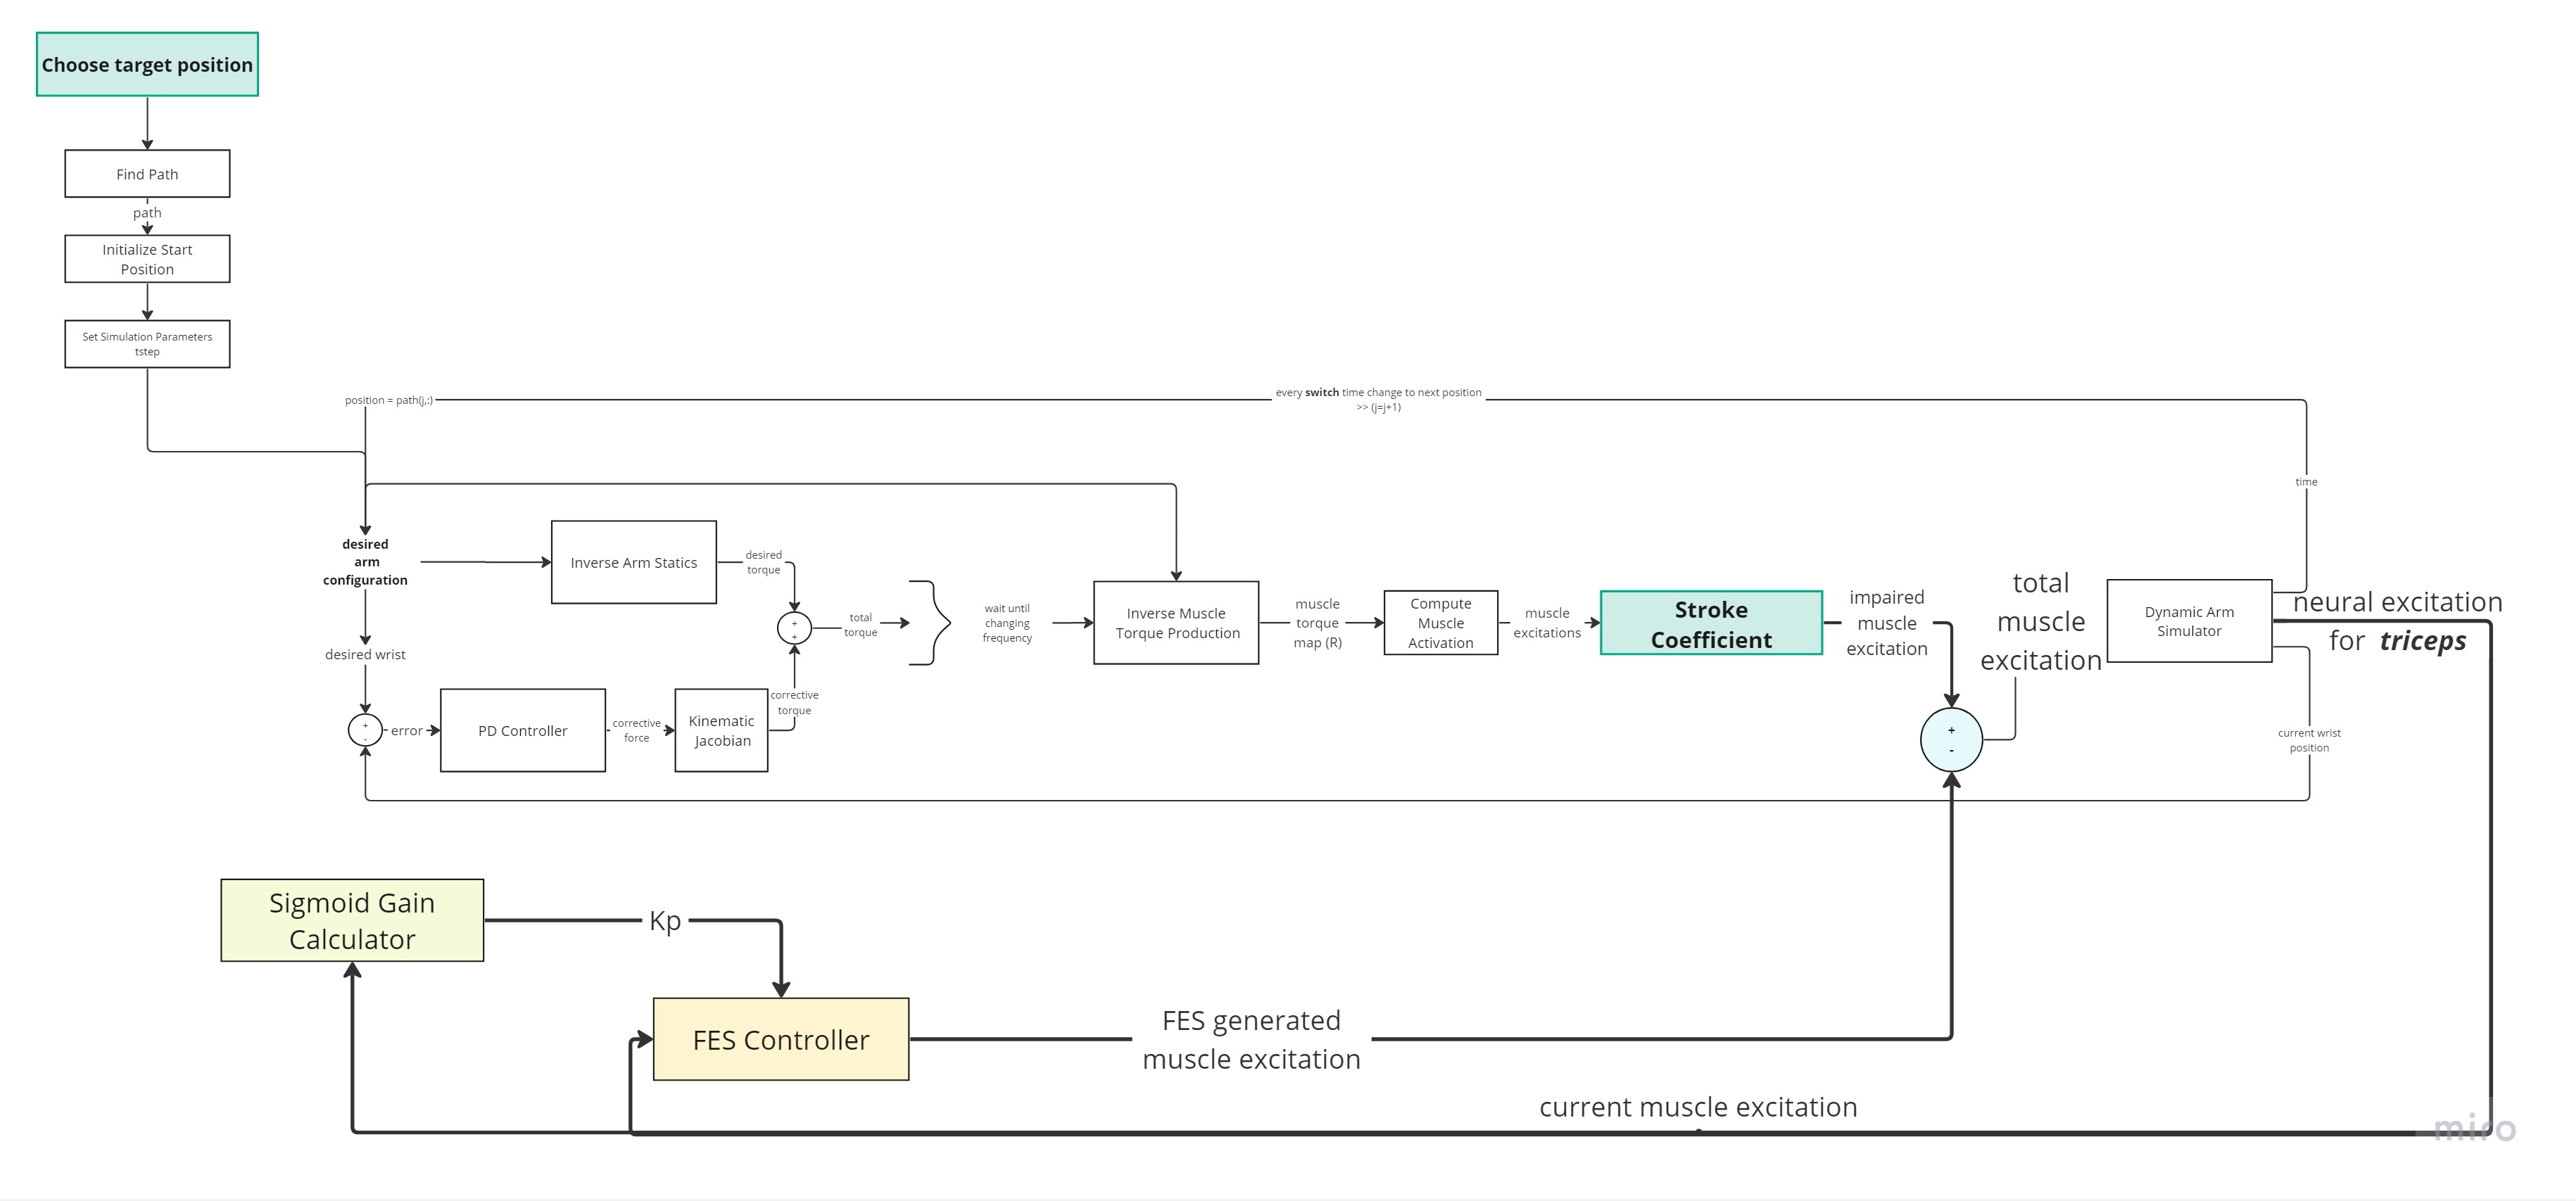
\includegraphics[width=1.7\textwidth]{Pictures/Controller/FESController.jpg} % Replace "filename.jpg" with the name of your image file
    \caption{Flow Diagram for EMG-influenced FES Controller} % Optional caption
    \label{fig:FESController} % Optional label for referencing
  \end{figure}
\end{landscape} % End landscape page

